\chapter{Ljós}

\begin{tcolorbox}

\iduck{Það fyrsta sem Newton komst að raun um þegar hann hóf að athuga ljós var að hvítt ljós er blanda lita. Með glerstrendingi gat hann klofið hvítt ljós í ýmsa liti, en þegar hann sendi einlitt ljós - til dæmis rautt - gegnum annan þrístrending sá hann að ekki var hægt að kljúfa það frekar. Newton uppgötvaði því að hvítt ljós er blanda lita sem eru hreinir í þeim skilningi að engan þeirra er hægt að kljúfa í sundur. Newton taldi ljós samanstanda af eindum og hann hafði rétt fyrir sér (en rökin hans voru röng). Við vitum að ljós samanstendur af ögnum því það eru til næm tæki sem gefa frá sér smelli ef ljós skín á þau, og þótt ljósið dofni meir og meir eru smellirnir alltaf jafn háir, aðeins færri. Ljós er því ekki óvsipað regndropum. Hver dropi ljóss er kallaður ljóseind og ef ljósið er einlitt eru allir droparnir jafn stórir.} \\

\vspace{-0.5cm}
\raggedleft{- \textbf{Richard P. Feynman, Ljósið, 1985}}
\end{tcolorbox}


\section{Lögmál Snells}

Ljós ferðast alltaf með hraða $c = \SI{3.00e8}{m/s}$ óháð viðmiðunarkerfi. Hinsvegar, þá segir fólk stundum óheppilega að ljós ferðist ,,hægar`` í sumum efnum. En það er einfaldlega vegna þess að ljósið virðist ferðast hægar því að sameindir efnisins sem að ljósið ferðast í gegnum gleypa ljóseindirnar sem að lenda í árekstri við þær. Við það örvast sameindir efnisins upp í hærra orkustig, en sameindirnar vilja að eðlisfari vera í orkulægsta ástandinu sínu, grunnástandinu, svo að þær geisla aftur orkunni í burtu (jafn mikil orka svo að ljósið sem losnar aftur hefur sömu tíðni og upphaflega ljósið hafði). Við þetta virðist hægjast á ljósinu því hver svona árekstur tekur um það bil \SI{1}{ns} (fer eftir því hversu þétt efnið er). Það sem meira er þá hefur þetta í för með sér að ljósgeislinn beygir við það að fara inn í önnur efni (hægt að sjá það með skriðþungavarðveislu á skilfletinum t.d.). Annað merkilegt, er eftirfarandi forsenda sem er gjarnan tileinkuð Fermat um eðli ljóssins:

\begin{tcolorbox}
\begin{theorem}
\textbf{(Lögmál Fermats)} Ljósið ferðast ávallt þá leið milli tveggja punkta sem tekur stystan tíma að ferðast.
\end{theorem}
\end{tcolorbox}


\begin{tcolorbox}
\begin{definition}
Við táknum með $n_{\text{efni}}$ brotstuðul efnis þar sem að ljóshraðinn er $c_{\text{efni}} < c$. Brotstuðullinn er skilgreindur þannig að:
\begin{align*}
    n_{\text{efni}} = \frac{c}{c_{\text{efni}}}
\end{align*}
\end{definition}
\end{tcolorbox}

Takið sér í lagi eftir því að við höfum ávallt að $n_{\text{efni}} \geq 1$ því $c_{\text{efni}} \leq c$.


\begin{comment}
\begin{table}[H]
    \centering
    \begin{tabular}{|l|c|}
    \hline
        Efni & $n$ \\ \hline \hline
       Tómarúm  & \num{1} \\ \hline
       Andrúmsloft  & \num{1.0003} \\ \hline
       Ís  & \num{1.31} \\ \hline
       Vatn  & \num{1.33} \\ \hline
       Etanól & \num{1.36} \\ \hline
       Olía  & \num{1.46} \\ \hline
       Gler  & \num{1.52} \\ \hline
       Akrýl  & \num{1.49} \\ \hline
       Demantur  & \num{2.41} \\ \hline
       German  & \num{4.00} \\ \hline
    \end{tabular}
    \caption{Brotstuðlar fyrir mismunandi efni.}
    \label{table:brotstudlar}
\end{table}
\end{comment}



\begin{tcolorbox}
\begin{theorem} \textbf{(Lögmál Snells)} Látum ljós ferðast á milli tveggja efna þar sem að brotstuðlarnir eru $n_1$ og $n_2$. Látum $\theta_1$ og $\theta_2$ vera hornin sem að ljósgeislinn myndar við þverlana. Þá gildir að:
\begin{minipage}{\linewidth}
\begin{wrapfigure}{r}{1.5in}
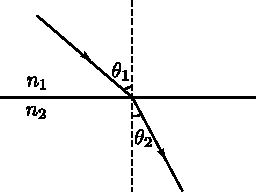
\includegraphics[width = 1.5in]{figures/snell1.pdf}
\end{wrapfigure}
\begin{align*}
    n_1 \sin\theta_1 = n_2 \sin\theta_2
\end{align*}
\vspace{1.4cm}
\end{minipage}
\end{theorem}
\end{tcolorbox}


\begin{minipage}{\linewidth}
\begin{wrapfigure}{r}{1.9in}
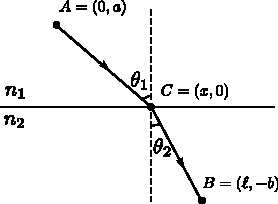
\includegraphics[width = 2.4in]{figures/snell2.pdf}
\end{wrapfigure}

\textbf{Útleiðsla 1:} Látum ljósgeislan byrja í $A = (0,a)$ og enda í $B = (\ell, -b)$ eftir viðkomu í $C = (x,0)$ á skilum efnanna. Við viljum lágmarka heildartímann sem það tekur ljósið að ferðast á milli $A$ og $C$. Þar sem að ljósið ferðast með hraða $c_1$ í efni $1$ en með hraða $c_2$ í efni 2 þá höfum við að heildartíminn sem það tekur ljósið að ferðast á milli $A$ og $C$ er gefinn með:
\begin{align*}
    \tau(x) = \frac{\sqrt{x^2+a^2}}{c_1} + \frac{\sqrt{\left( \ell - x \right)^2 + b^2}}{c_2}
\end{align*}
En samkvæmt Fermat velur ljósið þá leið sem að lágmarkar ferðatímann:
\begin{align*}
    \frac{d\tau}{dx} = \frac{x}{c_1\sqrt{x^2+a^2}} - \frac{\ell-x}{c_2 \sqrt{(\ell-x)^2+b^2}} \stackrel{!}{=} 0.
\end{align*}
\end{minipage}

\vspace{0.25cm}

En af skilgreiningunni á sínus sjáum við af rúmfræðinni á myndinni að:
\begin{align*}
    \sin\theta_1 = \frac{x}{\sqrt{x^2+a^2}}, \hspace{0.5cm} \text{og} \hspace{0.5cm} \sin\theta_2 = \frac{\ell-x}{\sqrt{(\ell-x)^2+b^2}}
\end{align*}
svo við ályktum að útgildið gefur að:
\begin{align*}
   \frac{d\tau}{dx} \stackrel{!}{=} 0 \implies \frac{\sin\theta_1}{c_1} = \frac{\sin\theta_2}{c_2}
\end{align*}
Við margföldum að lokum í gegn með ljóshraðanum $c$ og höfum því lögmál Snells:
\begin{align*}
            n_1 \sin\theta_1 = n_2 \sin\theta_2.
\end{align*}
\qed

Það er reyndar til önnur útleiðsla á lögmáli Snells sem er kennd við Newton (og kannski líka smá Einstein). Hún er eftirfarandi:

\textbf{Útleiðsla 2:} Samkvæmt Einstein þá samanstendur ljós af litlum ögnum sem við köllum ljóseindir. Hver ljóseind hefur orku $E_\gamma = hf = \frac{hc}{\lambda}$ þar sem $f$ er tíðni ljóssins og $\lambda$ er bylgjulengd þess. Fyrir massalausar agnir (eins og ljósið) þá gildir að skriðþungi ljóssins er $p_\gamma = \frac{E}{c} = \frac{hf}{c}$. Ef við ímmyndum okkur hvað gerist á skilfleti efnanna þá sjáum við fyrir okkur að það er enginn heildarkraftur í láréttu stefnuna svo að skriðþunginn í láréttu stefnuna er varðveittur. Hinsvegar er einhver kraftur í lóðréttu stefnuna á skilunum - við getum hugsað okkur að það sé vegna aðdráttarkraftsins frá sameindunum á sitt hvorri hliðinni. En skriðþungavarðveislan í láréttu stefnuna gefur strax lögmál Snells:
\begin{align*}
    \frac{hf_1}{c_1}\sin\theta_1 = \frac{hf_2}{c_2}\sin\theta_2
\end{align*}
þar sem að heildarorka ljóseindanna er varðveitt svo $hf_1 = hf_2$. Við margföldum loks í gegn með $c$ og fáum:
\begin{align*}
    n_1 \sin\theta_1 = n_2 \sin\theta_2.
\end{align*}
\qed

\section{Alspeglun}

Að lokum skulum við fjalla stuttlega um alspeglun. Skoðum aðeins lögmál Snells aftur:
\begin{align*}
    n_1 \sin\theta_1 = n_2 \sin\theta_2 \implies \sin\theta_2 = \frac{n_1}{n_2}\sin\theta_1
\end{align*}
Eina leiðin til þess að þessi jafna geti gengið er ef að stærðin:
\begin{align*}
    \frac{n_1}{n_2}\sin\theta_1 \leq 1
\end{align*}
Þá hefur jafnan alltaf lausn og $\theta_2$ ákvarðast af því skilyrði - með öðrum orðum þá kemst geislinn út úr efninu. Hinsvegar ef
\begin{align*}
    \frac{n_1}{n_2}\sin\theta_1 > 1
\end{align*}
þá fáum við svokallaða \textbf{alspeglun}. Þá sleppur geislinn ekki út um hina hliðina. Við sjáum líka að þar sem að $\sin\theta_1 \leq 1$ þá er eina leiðin til þess að fá alspeglun ef:
\begin{align*}
    \frac{n_1}{n_2} > 1 \implies n_1 > n_2.
\end{align*}
Með öðrum orðum þá sjáum við að alspeglun getur einungis orðið þegar að ljós fer úr efni með hærri brotstuðul í efni með lægri brotstuðul þ.e.a.s. úr þéttara efni í ekki eins þétt efni (t.d. gler í loft eða gler í vatn). \\

Sér í lagi sjáum við að ef að það verður speglun þá er innfallshornið $\theta_1$ jafnt útfallshorninu, $\theta_2$, þ.e.

\begin{figure}[H]
    \centering
    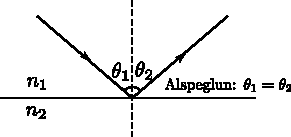
\includegraphics[scale = 1.5]{figures/snell3.pdf}
\end{figure}
Með öðrum orðum þá vitum við að þegar að hlutir speglast af yfirborði þá er $\theta_1 = \theta_2$.


\begin{comment}
\begin{figure}[H]
    \centering
    \begin{tikzpicture}[scale = 0.9]

    % define coordinates
    \coordinate (O) at (0,0) ;
    \coordinate (A) at (0,4) ;
    \coordinate (B) at (0,-4) ;
    
    % media
    \fill[blue!25!,opacity=.3] (-4,0) rectangle (4,4);
    \fill[blue!60!,opacity=.3] (-4,0) rectangle (4,-4);
    \node[left] at (-2,1) {$n_{2}$};
    \node[left] at (-2,-1) {$n_{1}$};

    % axis
    \draw[dash pattern=on5pt off3pt] (A) -- (B) ;

    % rays
    \draw[red,ultra thick,directed] (O) -- (50:4);
    \draw[blue,reverse directed,ultra thick] (O) -- (-110:3.5);
    %Punktar
    \filldraw[color=blue] (-110:3.5) circle (0.08) node[anchor=north, color=black] {$A(x_{1},y_{1})$};
    \filldraw[color=red] (50:4) circle (0.08)
    node[anchor=south, color=black] {$B(x_{2},y_{2})$};
    \filldraw[] (O) circle (0.08) node[anchor=west, color=black];
    % angles
    \draw (0,1) arc (90:50:1);
    \draw (0,-1.4) arc (270:250:1.4) ;
    \node[] at (260:1.8)  {$\theta_{1}$};
    \node[] at (70:1.4)  {$\theta_{2}$};
    \node[] at (-17:0.8) {$C(x,0)$};
\end{tikzpicture}

\end{figure}
\end{comment}

\section{Upprifjun: Einföld sveifluhreyfing og bylgjusamliðun}

Á þessu stigi málsins þá held ég að við þurfum að rifja upp aðeins úr $5.$ bekk. Til að byrja með skulum við rifja upp hvað einföld sveifluhreyfing er:

\begin{tcolorbox}
\begin{definition}
Við segjum að hlutur sé á \textbf{einfaldri sveifluhreyfingu} með \textbf{sveiflutíðni} $\omega$ ef lýsa má staðsetningu hlutarins, $z(t)$, sem fall af tíma með jöfnu af gerðinni:
\begin{align*}
    \Ddot{z} = - \omega^2z.
\end{align*}
\end{definition}
\end{tcolorbox}
Eins og þið munið síðar læra þá er þetta óhliðruð $2.$ stigs diffurjafna með fastastuðlum sem hefur lausn:
\begin{align*}
    x(t) = A\cos(\omega t + \varphi).
\end{align*}
Til þess að sanna að eitthvað fall sé lausn á diffurjöfnu þá diffrar maður einfaldlega fallið og sýnir að það uppfylli diffurjöfnuna. En við athugum einmitt að:
\begin{align*}
    \Dot{x}(t) =  \frac{dx}{dt} = -A\omega\sin(\omega t + \varphi), \hspace{1cm} \Ddot{x}(t) = \frac{d^2x}{dt^2} = -A\omega^2 \cos(\omega t + \varphi) = -\omega^2x(t)
\end{align*}
Sem sýnir að $x(t) = A\cos(\omega t + \varphi)$ er fullkomin lausn á diffurjöfnunni. Almennt þarf $2$ fasta (hér $A$ og $\varphi$) til þess að ákvarða fullkomlega lausn á $2.$ stigs diffurjöfnu. Bylgjur eru síðan bara tvær einfaldar sveifluhreyfingar settar saman í eina hreyfingu, þ.e.a.s~einföld sveifluhreyfing í tíma og rúmi. Bylgjujafnan er:
\begin{tcolorbox}
\begin{definition}
Látum $\psi(x,t)$ lýsa fráviki hlutar frá jafnvægisstöðu sinni sem fall af staðsetningu, $x$ og tíma, $t$. Við segjum að hluturinn sé á \textbf{bylgjuhreyfingu} með \textbf{bylgjuhraða} $c$ ef frávikið uppfyllir \textbf{bylgjujöfnuna}:
\begin{align*}
    \frac{\partial^2\psi}{\partial t^2} = c^2 \frac{\partial^2 \psi}{\partial x^2}
\end{align*}
\end{definition}
\end{tcolorbox}
Lausnir á bylgjujöfnunni eru þá föll af gerðinni:
\begin{align*}
    \psi(x,t) = A\sin(kx - \omega t + \varphi), \hspace{1cm} \text{þar sem} \hspace{1cm} \omega =  ck.
\end{align*}
Sem við getum auðveldlega sannað með diffrun:
\begin{align*}
    \frac{\partial^2\psi}{\partial t^2} = -\omega^2 \psi(x,t), \hspace{1cm} c^2\frac{\partial^2 \psi}{\partial x^2} = -c^2k^2\psi(x,t) = -\omega^2 \psi(x,t).
\end{align*}
Ef við leggjum síðan saman tvær samfasa bylgjur frá sömu uppsprettu (það þýðir í stuttu máli að tíðnin er sú sama og þar með bylgjulengdin þar að auki sem að fasahornið er núll og  þá höfum við:

\begin{tcolorbox}
\begin{theorem}
Hugsum okkur að við höfum tvær samfasa bylgjuuppsprettur í fjarlægð $d$ frá hvor annarri sem senda út eins bylgjur með útslag $A$, tíðni $f$ og bylgjulengd $\lambda$. Skoðum einhvern punkt, $P$, sem er þannig að önnur uppsprettan er í fjarlægð $r_1$ frá punktinum og hin uppsprettan er í fjarlægð $r_2$ frá punktinum.
\begin{figure}[H]
    \centering
    \vspace{-0.5cm}
    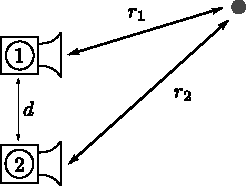
\includegraphics{figures/hatalari-dist.pdf}
\end{figure}
Þá er samliðunarbylgjan sem athugandi í punkti $P$ greinir gefin með:
\begin{align*} 
A\sin(kr_1-\omega t) + A\sin(kr_2 - \omega t) = 2A\cos(\frac{1}{2}k\Delta r)\sin(\frac{1}{2}k(r_1+r_2)-\omega t).
\end{align*}
Sér í lagi þá mun athugandinn heyra fullkomlega styrkjandi/eyðandi bylgjusamliðun í punkti $P$ ef:
\begin{align*}
    \Delta r = \begin{cases}
    n \lambda \hspace{2.8cm} \text{(styrkjandi bylgjusamliðun)} \\
    \left(n+\frac{1}{2}\right)\lambda \hspace{1.8cm} \text{(eyðandi bylgjusamliðun)}
    \end{cases},\hspace{1cm} n \in \N.
\end{align*}
\end{theorem}
\end{tcolorbox}

\textbf{Útleiðsla:} Skoðum samliðunarbylgjuna í punktinum $P$ en hún er gefin með:
\begin{align*}
    \psi_{\text{P}} = \psi_1 + \psi_2 = A \sin(k r_1 - \omega t) +  A \sin(k r_2 - \omega t)
\end{align*}
Með því að nota þáttunarreglur hornafalla:
\begin{align*}
    \sin(s) + \sin(t) = 2\sin(\frac{s+t}{2})\cos(\frac{s-t}{2}),
\end{align*}
fæst að:
\begin{align*}
    \psi &= A \sin(k r_1 - \omega t) +  A \sin(k r_2 - \omega t) \\
    &= 2A\sin(\frac{\left(kr_1 - \omega t\right) + \left(k r_2 -\omega t\right)}{2})\cos(\frac{\left( k r_1 - \omega t \right) - \left( kr_2 - \omega t \right)}{2}) \\
    &= 2A\cos(\frac{1}{2}k\Delta r)\sin(\frac{1}{2}k(r_1+r_2)-\omega t).
\end{align*}
Við sjáum að samliðunarbylgjan hegðar sér eins og bylgja með fast útslag $B = 2A\cos(\frac{1}{2}k\Delta r)$, tíðni $f$ og bylgjulengd $\lambda$, sem rita mætti sem $\psi = B\sin(kr - \omega t)$ þar sem $r =  \frac{r_1 + r_2}{2}$ er meðalfjarlægðin frá hátölurunum. En þá fæst fullkomlega styrkjandi bylgjusamliðun $B = 2A$ ef:
\begin{align*}
    \cos(\frac{1}{2}k\Delta r) = 1 \implies \frac{1}{2}k\Delta r = n\pi \implies \Delta r = \frac{2n\pi}{k} = n\lambda.
\end{align*}
En fullkomlega eyðandi bylgjusamliðun $B = 0$ ef:
\begin{align*}
    \cos(\frac{1}{2}k\Delta r) = 0 \implies \frac{1}{2}k\Delta r = \frac{\pi}{2} + n\pi = (2n+1)\frac{\pi}{2} \implies \Delta r = (2n +1)\frac{\pi}{k} = \left(n + \frac{1}{2}\right)\lambda.
\end{align*}
Almennt segjum við að samliðun sé \textbf{styrkjandi} ef $B > A$ og \textbf{eyðandi} ef $B < A$. \qed



\section{Tveggja raufa tilraun Youngs: Ljóssamliðun}

Nú komum við að tveggja raufa tilraun Youngs sem var fyrst notuð til þess að sýna fram á bylgjueðli ljóss. Þá er leisigeisla með bygljulengd $\lambda$ beint í gegnum tvær raufar eins og á myndinni hér fyrir neðan. Þá kemur fram styrkjandi bylgjusamliðun á skjá fyrir aftan raufarnar.

\begin{figure}[H]
    \centering
    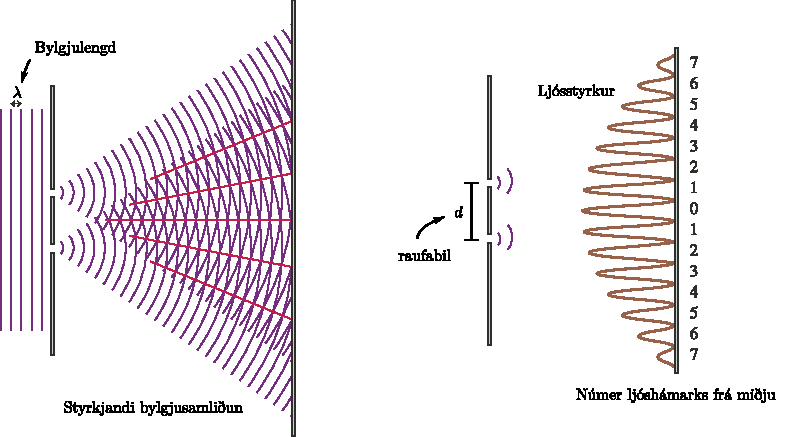
\includegraphics[scale = 0.9]{figures/young-double.pdf}
\end{figure}


\begin{tcolorbox}
\begin{theorem}
Þegar leisigeisla með bylgjulengd $\lambda$ er beint í gegnum tvær raufar með raufabil $d$ þá kemur fram styrkjandi samliðunarmynstur í fjarlægð $\ell$ fyrir aftan raufarnar. Ef $y_n$ táknar staðsetningu björtu ljóshámarkanna þá gildir að:
\begin{align*}
    d\sin\theta_n = n\lambda, \hspace{1cm} y_n = \ell \tan\theta_n
\end{align*}
Sér í lagi ef $\theta_n \ll 1$ þá gildir að bilið á milli ljósráka á skjánum er með góðri nálgun fast:
\begin{align*}
    \Delta y = \frac{\lambda \ell}{d}
\end{align*}
\end{theorem}
\end{tcolorbox}

\textbf{Útleiðsla 1:} Til þess að bylgjusamliðunin sé styrkjandi í punkti á skjánum í fjarlægð $y_n$ frá miðjunni þá þarf að muna heiltölumargfeldi af bylgjulengdum á vegalengdinni sem að geislarnir þurfa að ferðast frá hvorri rauf þannig að $\Delta r = n\lambda$. En við sjáum af eftirfarandi mynd:

\begin{figure}[H]
    \centering
    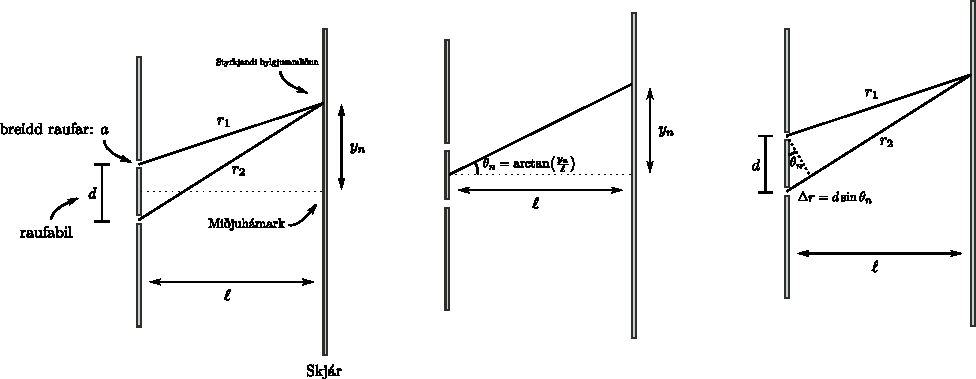
\includegraphics{figures/young-diagram.pdf}
\end{figure}

Við ályktum þar með að 

\begin{align*}
    d\sin\theta_n = \Delta r = n \lambda
\end{align*}
Þar að auki sem að rúmfræðilega staðsetning ljóshámarksins gefur okkur að:
\begin{align*}
    y_n = \ell \tan\theta_n
\end{align*}

Sér í lagi ber að nefna að ef $\theta_n \ll 1$ þá er $\sin\theta_n \approx \theta_n$ og $\tan\theta_n \approx \theta_n$ svo að fyrir lítil horn gildir að:
\begin{align*}
    y_n = \ell \tan\theta_n \approx \ell \sin\theta_n = \frac{n\lambda \ell}{d} \implies \Delta y = y_{n+1} - y_n = \frac{\lambda \ell}{d}.
\end{align*}
\qed



\textbf{Útleiðsla 2:} Ef að manni finnst þetta vera frekar óformlegt (eins og mér) og maður er ekki sannfærður á þessum rökum (eins og ég) þá gæti maður vilja gera þetta aðeins formlegra. Athugum fyrst að:
\begin{align*}
    \sin\theta_n = \frac{y_n}{\sqrt{\ell^2 + y_n^2}}.
\end{align*}
Höfum síðan að mismunurinn á vegalengdinni sem að ljósið þarf að ferðast er:
\begin{align*}
   n\lambda = \Delta r = r_2 - r_1 = \sqrt{\ell^2 + \left(y_n+\frac{d}{2}\right)^2} - \sqrt{\ell^2 + \left(y_n-\frac{d}{2}\right)^2}
\end{align*}
Með því að margfalda með samokastærðinni sjáum við að:
\begin{align*}
    n\lambda = \frac{\left(y_n + \frac{d}{2} \right)^2 - \left( y_n - \frac{d}{2} \right)^2}{\sqrt{\ell^2 + \left(y_n+\frac{d}{2}\right)^2} + \sqrt{\ell^2 + \left(y_n-\frac{d}{2}\right)^2}} = \frac{2y_n d}{\sqrt{\ell^2 + \left(y_n+\frac{d}{2}\right)^2} + \sqrt{\ell^2 + \left(y_n-\frac{d}{2}\right)^2}} \stackrel{y_n \gg \frac{d}{2}}{\approx} \frac{y_n d}{\sqrt{\ell^2 + y_n^2}} = d\sin\theta_n.
\end{align*}
Sér í lagi sést í þessari nálgun að ef þar að auki við höfum að $\ell \gg y_n$ þá er þar að auki:
\begin{align*}
    n \lambda \stackrel{y_n \gg \frac{d}{2}}{\approx} \frac{y_n d}{\sqrt{\ell^2 + y_n^2}} \stackrel{\ell \gg y_n}{\approx} \frac{y_n d}{\ell} \implies y_n = \frac{n\lambda \ell}{d}.
\end{align*}
\qed

\section{Margar raufar}

Helsti kosturinn við seinni útleiðsluna hér á undan er að þá sér maður að svo lengi sem að $y_n \gg \frac{d}{2}$ þá mun $d\sin\theta_n = n\lambda$ gilda. Þá sjáum við að ef við höfum ljósgreiðu með mörgum raufum þá munu raufabilin sem eru hlið við hlið alltaf gefa sömu niðurstöðu og fyrir tveggja raufa mynstrið. Fyrir margar raufar þá er raufabilið oftast minna svo það dreifist meira úr ljóshámörkunum á skjánum en það þýðir að seinni nálgunin $\ell \gg y_n$ gildir ekki. Þar með höfum við:
\begin{figure}[H]
    \centering
    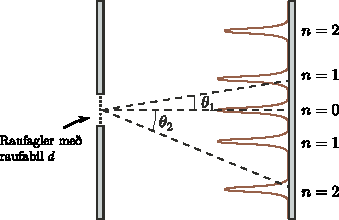
\includegraphics{figures/manyslits.pdf}
\end{figure}

\begin{tcolorbox}
\begin{theorem}
Þegar að leisigeisla með bylgjulengd $\lambda$ er beint í gegnum ljósgreiðu með raufabil $d$ þá kemur fram styrkjandi samliðunarmynstur á skjá í fjarlægð $\ell$ fyrir aftan raufaglerið. Ef $y_n$ táknar staðsetningu björtu ljóshámarkanna þá gildir að:
\begin{align*}
    d\sin\theta_n = n\lambda, \hspace{1cm} y_n = \ell \tan\theta_n
\end{align*}
\end{theorem}
\end{tcolorbox}

\section{Ein rauf: Ljósbognun}

Ef við setjum fyrir aðra raufina þannig að leisigeislinn kemst bara út um aðra raufina þá fáum við svokallað ljósbognunarmynstur.

\begin{figure}[H]
    \centering
    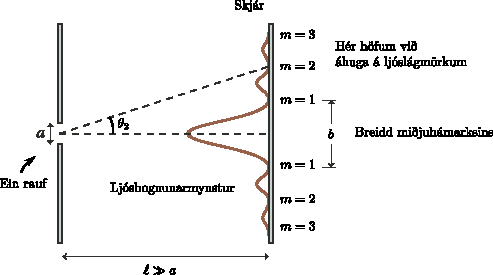
\includegraphics{figures/ljosbognun.pdf}
\end{figure}

\begin{tcolorbox}
Þegar að leisigeisla með bylgjulengd $\lambda$ er beint í gegnum eina rauf af stærð $a$ þá kemur fram ljósbognunarmynstur á skjá í fjarlægð $\ell$ fyrir aftan. Ef $y_n$ táknar staðsetningu dökku rákana (ljóslággildin) þá gildir að:
\begin{align*}
    a\sin\theta_n = n\lambda, \hspace{1cm} y_n = \ell \tan\theta_n
\end{align*}
Að því gefnu að $\theta_1 \ll 1$ þá höfum við að breiddin á miðjuhámarkinu, $b$, er gefin með:
\begin{align*}
    b = \frac{2\lambda \ell}{a}.
\end{align*}
\end{tcolorbox}


\section{Bæði samliðunarmynstur og bognunarmynstur}

Í flestum tilvikum þá fáum við hinsvegar fram bæði mynstrin í einu (því það er óhjákvæmilegt að ef við erum með margra raufagler að raufarnar hafi ekki einhverja þykkt $a$ og eitthvað raufabil $d$). En hvernig lítur slíkt mynstur út? Það er í rauninni bara bæði mynstrin sett saman í eitt. Hér er til dæmis mynd til útskýringar:

\begin{figure}[H]
    \centering
    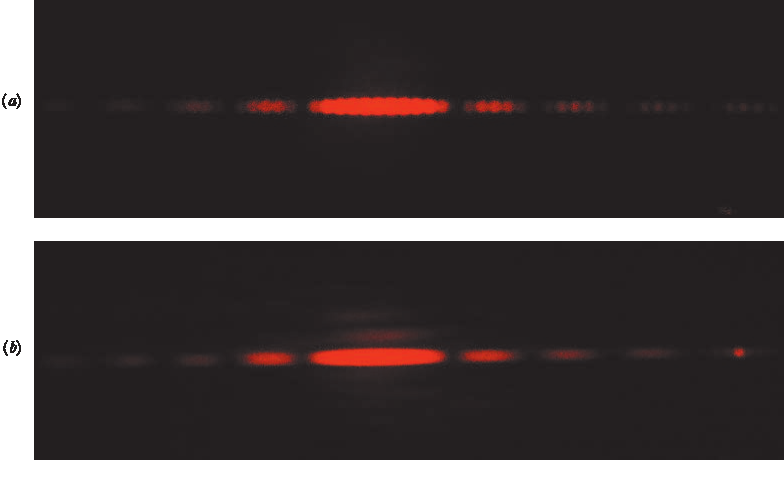
\includegraphics[scale = 0.9]{figures/jearl-walker.pdf}
\end{figure}
Á mynd (a) hér að ofan sést hefðbundið samliðunarmynstur fyrir tveggja raufa raufagler. En samliðunarmynstrið samanstendur í rauninni af tveimur mynstrum. Því á mynd (b) sést mynstrið sem fæst þegar að við lokum fyrir aðra raufina þannig að ljósið kemst bara í gegnum eina rauf. Þá sjáum við að dökku rákirnar koma útaf því hversu breið hver rauf er en ljóshámörkin inni í miðjuhámarkinu er vegna þess hversu langt er á milli ljóshámarkanna (sér í lagi gildir 
á þessum myndum að $\lambda < a < d $). Mynstrið sem kemur fram verður þá einhvern veginn svona:

\begin{figure}[H]
    \centering
    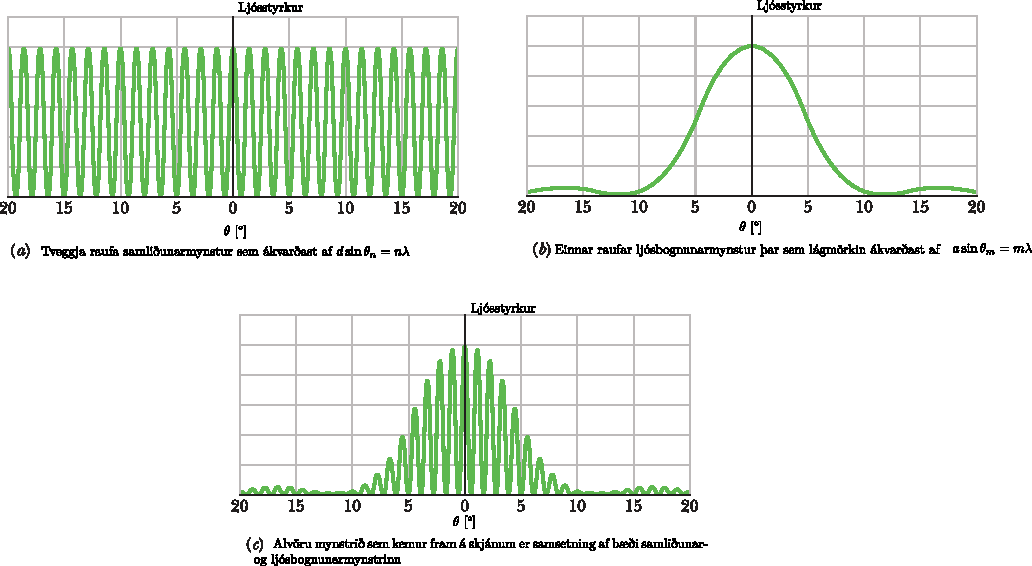
\includegraphics{figures/samlidun.pdf}
\end{figure}


\section{Linsur og geislagangsmyndir}

Linsur eru algengar í daglegu lífi. Þær er að finna í sjónaukum, smásjám og myndavélum þar að auki sem að þær eru megingrundvöllurinn fyrir því hvernig að gleraugu og augnlinsur virka (sumir nota slíkt á hverjum degi!). Til að byrja með skulum við setja fram tvær helstu gerðir af linsum sem að fólk notar:

\begin{tcolorbox}
\begin{definition} Við segjum að linsa sé:
\begin{enumerate}[label = \textbf{(\roman*)}]
    \item \textbf{Safnlinsa} ef allir geislar sem ferðast samsíða í gegnum linsuna safnast saman í einum \textbf{brennipunkti} í fjarlægð $f$ frá linsunni á ás linsunnar.
    \item \textbf{Dreifilinsa} ef allir geislar sem ferðast samsíða í gegnum linsuna tvístrast burt frá ás linsunnar eins og að þeir hafi komið úr brennipunktinum í fjarlægð $-f$ frá linsunni.
\end{enumerate}
\begin{figure}[H]
    \centering
    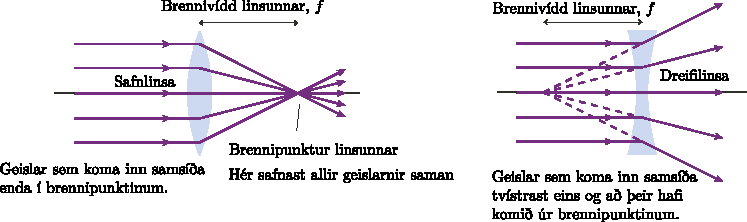
\includegraphics{figures/dreifi-safn.pdf}
\end{figure}
Talan $f$ kallast \textbf{brennivídd} linsunnar. Safnlinsur hafa jákvæða brennivídd en dreifilinsur hafa neikvæða brennivídd.
\end{definition}
\end{tcolorbox}

Það ber að nefna að á hinni hlið linsunnar er alltaf alveg eins brennipunktur í sömu fjarlægð.

\section{Safnlinsur: Raunveruleg mynd}

\begin{tcolorbox}
\begin{theorem}
Lítum á hlut með hæð $h$ sem stendur í fjarlægð $a$ frá safnlinsu með brennivídd $f$ þar sem $a>f$. Þá kemur fram skörp, viðsnúin raunmynd í fjarlægð $b$ hinum meginn við linsuna þar sem að hæð eftirmyndarinnar verður $H = \frac{b}{a}h$ þar að auki sem að við höfum \textbf{linsujöfnuna}:
\begin{align*}
    \frac{1}{a} + \frac{1}{b} = \frac{1}{f}
\end{align*}
\begin{figure}[H]
    \centering
    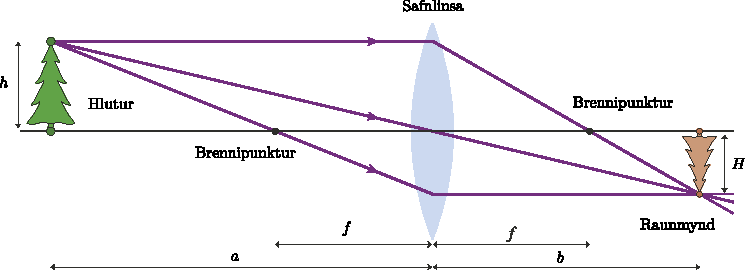
\includegraphics{figures/safnlinsa-raunmynd.pdf}
\end{figure}
\end{theorem}
\end{tcolorbox}

\textbf{Útleiðsla:} Látum hæð hlutarins vera $h$ og hæð eftirmyndarinnar vera $H$. Jafna línunnar sem að tengir saman punktana $(0,h)$ og $(f,0)$ er gefin með:
\begin{align*}
    y - h = \left( \frac{h-0}{0-f} \right)(x-0), \hspace{0.5cm} \text{þ.e.} \hspace{0.5cm} y_1 = h - \frac{h}{f}x
\end{align*}
Hinsvegar, þá er jafna línunnar sem að liggur milli $(-a,h)$ og $(b,-H)$ gefin með:
\begin{align*}
    y-h = \left( \frac{-H-h}{b-(-a)} \right)(x-(-a)), \hspace{0.5cm} \text{þ.e.} \hspace{0.5cm} y_2 = h - \left( \frac{H+h}{a+b} \right)(x+a).
\end{align*}
Við vitum að seinni línan fer í gegnum $(0,0)$. Athugum að skilyrðið $y_2(0) = 0$ gefur því að:
\begin{align*}
    y_2(0) = 0 &\implies h - \left( \frac{H+h}{a+b} \right)a = 0 
    \implies h(a+b) = (H+h)a 
    \implies hb = Ha 
    \implies \frac{H}{h} = \frac{b}{a}.
\end{align*}
Svo við ályktum að $\frac{b}{a}$ lýsir stækkun myndarinnar:
\begin{align*}
    H = \frac{b}{a}h
\end{align*}
Sér í lagi sjáum við að ef $b>a$ þá stækkar myhndin en ef $a>b$ þá minnkar myndin. Við viljum síðan að línurnar $y_1$ og $y_2$ skerist í $x=b$. Við höfum því að:
\begin{align*}
    y_1(b) = y_2(b) &\implies h - \frac{h}{f}b = h- \frac{H+h}{a+b}\left(a+b\right) = -H \\
    &\implies 1 - \frac{b}{f} = -\frac{H}{h} = -\frac{b}{a} \\
    &\implies \frac{1}{b} - \frac{1}{f} = -\frac{1}{a}
\end{align*}
Sem gefur því að lokum linsujöfnuna:
\begin{align*}
    \frac{1}{a} + \frac{1}{b} = \frac{1}{f}.
\end{align*}
\qed

\section{Safnlinsur: Ímynduð mynd}

Við skulum líka skoða hvað gerist ef hluturinn okkar er fyrir innan brennipunktinn. Það er að segja ef að $a < f$. Eina leiðin til þess að linsujafnan:
\begin{align*}
    \frac{1}{a} + \frac{1}{b} = \frac{1}{f}
\end{align*}
gangi upp með $a < f$, þ.e.~$\frac{1}{a} > \frac{1}{f}$ er ef að $b$ er neikvæð! En það samsvarar því að myndin kemur fram sömu meginn og hluturinn nema fyrir utan brennipunktinn, $b > f$. Við höfum semsagt:

\begin{tcolorbox}
\begin{theorem}
Lítum á hlut með hæð $h$ sem stendur í fjarlægð $a$ frá safnlinsu með brennivídd $f$ þar sem $a < f$. Þá kemur fram skörp, ímynduð mynd í fjarlægð $b < 0$ sömu meginn við linsuna þar sem að hæð eftirmyndarinnar verður $H = \abs{\frac{b}{a}}h$ þar að auki sem að við höfum \textbf{linsujöfnuna}:
\begin{align*}
    \frac{1}{a} + \frac{1}{b} = \frac{1}{f}
\end{align*}
\begin{figure}[H]
    \centering
    \includegraphics{figures/imynduð-safnlinsa.pdf}
\end{figure}
\end{theorem}
\end{tcolorbox}

\textbf{Útleiðsla:} Þetta leiðir beint af útleiðslunni hér á undan nema maður ætti að benda á að hér er $b$ neikvætt.

\qed

Reyndar eitt sem er áhugavert er að við getum notað linsujöfnuna til að sýna að ímyndaða myndin sem kemur fram er alltaf stærri heldur en upphaflegi hluturinn. Athugum að linsujafnan gefur að:
\begin{align*}
    \frac{1}{a} + \frac{1}{b} = \frac{1}{f} \implies b = \left( \frac{1}{f} - \frac{1}{a} \right)^{-1} = \frac{af}{a-f} \implies \frac{b}{a} = -\frac{f}{f-a}
\end{align*}
og þar sem að $f > f-a$ þá er $\abs{\frac{b}{a}} > 1$ svo myndin stækkar alltaf.


\section{Dreifilinsur}

Að lokum skulum við fjalla stuttlega um dreifilinsur. Dreifilinsur eru áhugaverðar að því leitinu til að við fáum bara eitt tilvik (en ekki tvö eins og fyrir safnlinsuna. Fyrir dreifilinsur gildir líka linsujafnan nema núna er brennivídd linsunnar neikvæð $f < 0$ og við fáum alltaf ímyndaða mynd svo $b < 0$.

\begin{tcolorbox}
\begin{theorem}
Lítum á hlut með hæð $h$ sem stendur í fjarlægð $a$ frá dreifilinsu með brennivídd $f < 0$. Þá kemur fram skörp, smækkuð, ímynduð mynd í fjarlægð $b < 0$ sömu meginn við linsuna þar sem að hæð eftirmyndarinnar verður $H = \abs{\frac{b}{a}}h$ þar að auki sem að við höfum \textbf{linsujöfnuna}: $ \frac{1}{a} + \frac{1}{b} = \frac{1}{f}$.

\begin{figure}[H]
    \centering
    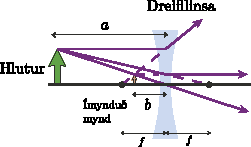
\includegraphics{figures/dreifilinsa.pdf}
\end{figure}
\end{theorem}
\end{tcolorbox}

\newpage

\section{Dæmi}

\subsection*{Dæmatími 39: Tveggja raufa tilraun Youngs}

\begin{tcolorbox}
\begin{minipage}{\linewidth}
\begin{wrapfigure}{r}{2.3in}
\vspace{-0.5cm}
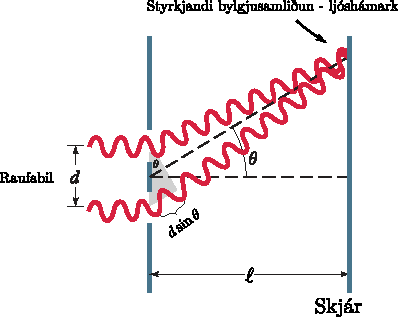
\includegraphics[width = 2.3in]{figures/young-raufar.pdf}
\end{wrapfigure}
Þegar leisigeisla með bylgjulengd $\lambda$ er skotið í gegnum tvær (eða fleiri) raufar þar sem að bilið á milli raufanna er $d$ þá kemur fram samliðunarmynstur á skjá í fjarlægð $\ell$ fyrir aftan. Fyrir slík mynstur þá höfum við áhuga á \textbf{ljóshámörkum} en rúmfræðilega er staðsetning ljóshámarkanna, $y_n$, gefin með:
\begin{align*}
    y_n = \ell \tan\theta_n
\end{align*}
Til þess að fá styrkjandi bylgjusamliðun, þá þarf mismunurinn á vegalengdinni sem að ljósið ferðast frá raufunum að vera jafnt heiltölufjölda bylgjulengda sem gefur okkur:
\begin{align*}
   d\sin\theta_n = n \lambda
\end{align*}
Fyrir lítil horn, $\theta \ll 1$, gildir að $\sin\theta \approx \theta$ og $\tan\theta \approx \theta$ svo $\tan\theta \approx \sin\theta$, en þá er:
\begin{align*}
    y_n = \ell \tan\theta_n \approx \ell \sin\theta_n = \frac{n  \lambda \ell}{d} \implies \Delta y = \frac{\lambda \ell }{d}.
\end{align*}
\end{minipage}
\end{tcolorbox}

\begin{enumerate}[label = \textbf{(\alph*)}]

\item[\textbf{(33.2)}] Leisigeisla með bylgjulengd $\SI{600}{nm}$ er beint í gegnum tvær raufar með raufabil $\SI{50}{\mu m}$. Hvaða horn mun þriðja ljóshámarkið mynda miðað við upphaflegu stefnu leisigeislans?

\item[\textbf{(33.3)}] Leisigeisla með bylgjulengd $\SI{500}{nm}$ er beint í gegnum tvær raufar með óþekkt raufabil. Samliðunarmynstur sést fyrir aftan á skjá sem er í fjarlægð \SI{50}{cm} frá raufaglerinu. Fjarlægðin á milli björtu ljósrákanna á skjánum er \SI{2.5}{mm}. \begin{enumerate*}[label = \textbf{(\alph*)}]
    \item Hvert er raufabil raufaglersins?
    \item Hvert verður bilið á milli ljósrákanna á skjánum ef að leisigeisla með bylgjulengd \SI{600}{nm} er beint í gegnum raufaglerið?
\end{enumerate*}

\begin{minipage}{\linewidth}
\begin{wrapfigure}{r}{1.2in}
\vspace{-0.5cm}
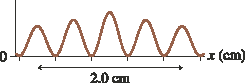
\includegraphics[width = 1.5in]{figures/rk3336.pdf}
\end{wrapfigure}

\item[\textbf{(33.37)}] Leisigeisla með óþekkta bylgjulengd er beint í gegnum tveggja raufa raufagler með raufabil \SI{0.20}{mm}. Á myndinni hér til hægri sést samliðunarmynstrið sem kom fram á skjá, \SI{2.0}{m}, fyrir aftan raufaglerið (grafið sýnir ljósstyrk sem fall af staðsetningu). Hver var bylgjulengd ljóssins?

\end{minipage}

\item[\textbf{(33.35)}] Leisigeisla með bylgjulengd $\SI{633}{nm}$ er beint í gegnum tveggja raufa raufagler með óþekkt raufabil. Samliðunarmynstur kemur fram á skjá \SI{3.0}{m} fyrir aftan raufaglerið. Þrettán bjartar rákir sjást á skjánum fyrir aftan og heildarvegalengdin á milli ystu rákanna á skjánum er \SI{52}{mm}. Hvert er raufabilið?



\end{enumerate}

\begin{tcolorbox}
\begin{enumerate*}[label = ]
  \item \textbf{(33.2)} $\ang{2.06}$.
  \item \textbf{(32.3)} $\SI{100}{\mu m}$, $\SI{3.0}{mm}$.
  \item \textbf{(33.37)} $\SI{500}{nm}$.
  \item \textbf{(32.35)} $\SI{438}{\mu m}$.
\end{enumerate*}
\end{tcolorbox}

\newpage

\subsection*{Dæmatími 40: Ein rauf eða margar raufar?}

\begin{tcolorbox}
Fyrir margar raufar þá gilda sömu jöfnur fyrir \textbf{ljóshámörkin} og í dæmakafla 39. Hinsvegar fyrir eina rauf af breidd $a$ þá gilda sömu jöfnur og í dæmakafla 39 nema núna eru þær fyrir \textbf{ljóslágmörkin}:
\begin{align*}
    y_m = \ell \tan\theta_m, \hspace{1cm} a\sin\theta_m = m \lambda.
\end{align*}
\end{tcolorbox}

\begin{enumerate}[label = \textbf{(\alph*)}]

\item[\textbf{(33.13)}] Vetni hefur tvær sýnilegar litrófslínur, annars vegar rauða (\SI{656}{nm}) og hinsvegar bláa (\SI{486}{nm}). Ljósinu frá vetnislampa er nú beint í gegnum raufagler sem hefur \SI{500}{raufar/mm} og samliðunarmynstrið er skoðað á skjá \SI{1.50}{m} fyrir aftan raufaglerið. \begin{enumerate*}[label = \textbf{(\alph*)}]
    \item Hvert er raufabil raufaglersins?
    \item Þar sem að bylgjulengdir vetnislampans eru tvær sjást tvö samliðunarmynstur á skjánum. Hversu langt er bilið á milli fyrstu ljóshámarkanna frá bláa og rauða ljósinu?
\end{enumerate*}

\item[\textbf{(33.46)}] Sprengju-Kata er að skoða litrófslínur frá óþekktri efnablöndu. Hún hitar efnablönduna upp þannig að hún byrjar að geisla frá sér ljósi sem að hún beinir síðan í gegnum raufagler og skoðar ljóshámörkin á skjá \SI{15.0}{cm} fyrir aftan raufaglerið. Því miður týndi Katrín miðanum sem að segir til um raufabilið á raufaglerinu. Hinsvegar, þá er hún með aðra þekkta efnablöndu, sem að hún veit að geislar frá sér ljósi með bylgjulengd $\SI{461}{nm}$. Þegar að hún beinir ljósinu í gegn frá þekktu efnablöndunni þá sér hún bjarta litrófslínu í \SI{9.95}{cm} fjarlægð frá miðjunni. Hver er bylgjulengd ljóssins sem að óþekkta sýnið sendir frá sér ef að hún greinir litrófslínur þess í \SI{12.15}{cm} fjarlægð frá miðjunni?

\item[\textbf{(33.16)}] Leisigeisla með bylgjulengd $\SI{633}{nm}$ er beint í gegnum eina rauf með óþekkta breidd. Ljósbognunarmynstrið er skoðað á skjá \SI{1.5}{m} fyrir aftan raufina. Fjarlægðin á milli fyrsta og annars ljóslágmarksins er \SI{4.75}{mm}. Hver er breidd raufarinnar?

\begin{minipage}{\linewidth}
\begin{wrapfigure}{r}{1.2in}
\vspace{-0.5cm}
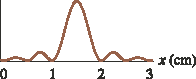
\includegraphics[width = 1.5in]{figures/rk3318.pdf}
\end{wrapfigure}

\item[\textbf{(33.17)}] Leisigeisla með bylgjulengd \SI{633}{nm} er beint í gegnum eina rauf með raufabil \SI{0.15}{mm}. Á myndinni hér til hægri sést ljósbognunarmynstrið sem kom fram á skjá fyrir aftan raufaglerið (grafið sýnir ljósstyrk sem fall af staðsetningu). Hversu langt fyrir aftan raufina er skjárinn?

\end{minipage}

\end{enumerate}

\begin{tcolorbox}
\begin{enumerate*}[label = ]
  \item \textbf{(33.13)} $\SI{14.5}{cm}$.
  \item \textbf{(33.46)} $\SI{525}{nm}$.
  \item \textbf{(33.16)} $\SI{200}{\mu m}$.
  \item \textbf{(32.17)} $\SI{1.18}{m}$.
\end{enumerate*}
\end{tcolorbox}

\newpage

\subsection*{Dæmatími 41: Lögmál Snells}

\begin{tcolorbox}
\begin{minipage}{\linewidth}
\begin{wrapfigure}{r}{1.5in}
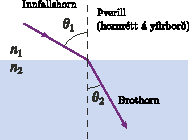
\includegraphics[width = 1.5in]{figures/snell.pdf}
\end{wrapfigure}
Ljós virðist ferðast hægar í mismunandi efnum heldur en í tómarúmi. Brotstuðull efnis er mælikvarði á hraða ljóss og er skilgreindur sem:
\begin{align*}
    n_{\text{efni}} = \frac{c}{c_{\text{efni}}}
\end{align*}
Lögmál Snells segir síðan að:
\begin{align*}
    n_1 \sin\theta_1 = n_2 \sin\theta_2
\end{align*}
\end{minipage}
\end{tcolorbox}

\begin{enumerate}[label = \textbf{(\alph*)}]

\item[\textbf{(34.10)}] Leisigeisla er beint inn í óþekktan vökva. Stefna geislans er þannig að leisigeislinn myndar \ang{45} innfallshorn. Við tökum eftir því að brothornið er \ang{30}. Hver er brotstuðullinn?

\vspace{0.5cm}

\begin{minipage}{\linewidth}
\begin{wrapfigure}{r}{1.5in}
\vspace{-0.5cm}
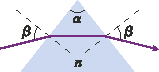
\includegraphics[width = 1.5in]{figures/vikhorn.pdf}
\end{wrapfigure}

\item[\textbf{(34.58)}] Á myndinni hér til hægri má sjá prisma með topphorn $\alpha$. Til er innfalshorn, $\beta$, sem er þannig að geislinn ferðast samhverft í gegnum prismað eins og sést á myndinni hér til hægri. \begin{enumerate*}[label = \textbf{(\alph*)}]
    \item Ákvarðið hornið $\beta$ sem fall af topphorninu, $\alpha$ og brotstuðlinum, $n$.
    \item Slúbbertar í ónefndum bekk eru að skoða vikhornsmælingar á prisma með topphorn $\alpha = \ang{60.0}$ og finna $\beta = \ang{52.2}$. Hver er brotstuðull prismans?
\end{enumerate*}

\vspace{0.5cm}

\begin{minipage}{\linewidth}
\begin{wrapfigure}{r}{1.2in}
\vspace{-0.5cm}
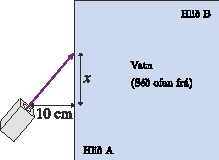
\includegraphics[width = 1.2in]{figures/rk3354.pdf}
\end{wrapfigure}

\item[\textbf{(34.54)}] Á myndinni hér til hægri sést leisigeisli í \SI{10}{cm} fjarlægð frá fiskabúri sem er fyllt með vatni (séð ofan frá). Brotstuðull vatns er $n_{\text{vatn}} = \num{1.33}$. Leisigeislanum er til að byrja með beint að fiskabúrinu þannig að $x = \SI{15}{cm}$.  \begin{enumerate*}[label = \textbf{(\alph*)}]
    \item Hvert er innfallshorn leisigeislans í vatnið?
    \item Hvert er brothornið?
    \item Þegar að geislinn lendir á hlið $B$ á myndinni, mun hann þá komast út úr fiskabúrinu eða endurkastast hann aftur inn í fiskabúrið?
    \item Endurtakið alla reikningana, nema núna fyrir $x = \SI{25}{cm}$.
    \item Hvert er minnsta gildið á $x$ þannig að geislinn sleppi út um $B$?
\end{enumerate*}

\end{minipage}


\begin{comment}
\vspace{2cm}

\begin{minipage}{\linewidth}
\begin{wrapfigure}{r}{1.2in}
\vspace{-0.5cm}
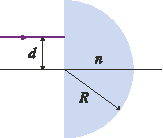
\includegraphics[width = 1.2in]{figures/rk3316.pdf}
\end{wrapfigure}

\item[\textbf{(33.16)}] Á myndinni hér til hægri má sjá hálfhring með geisla $R$ og brotstuðul $n$. Hver er mesta fjarlægðin, $d$, frá miðju hringsins sem að hægt er að varpa leisigeisla 



\end{minipage}
\end{comment}





\end{minipage}

\vspace{0.5cm}

\begin{minipage}{\linewidth}
\begin{wrapfigure}{r}{2in}
\vspace{-0.5cm}
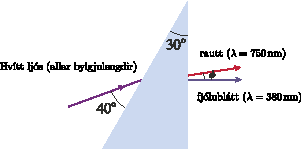
\includegraphics[width = 2.5in]{figures/rk3441.pdf}
\end{wrapfigure}

\item[\textbf{(35.41)}] ,,The Dark Side of The Moon`` eftir hljómsveitina Pink Floyd skartar einu frægasta plötuumslagi allra tíma. En á því má sjá svokallaða ljóstvístrun. Því ólíkt umfjölluninni okkar hingað til þá er brotstuðullinn reyndar háður bylgjulengd ljósins. Í þessu tiltekna dæmi getum við sagt að brotstuðullinn fyrir fjólublátt ljós er \SI{2}{\percent} meiri heldur en brotstuðullinn fyrir rautt ljós. Á myndinni hér til hægri sést slík ljóstvístrun þar sem að regnbogi myndast eftir að hvítt ljós fellur inn í prismað. Fjólublái geislinn er hornréttur á yfirborð prismans. Hvaða horn, $\phi$, er á milli rauða og fjólubláa ljóssins?



\end{minipage}

\end{enumerate}

\begin{tcolorbox}
\begin{enumerate*}[label = ]
  \item \textbf{(34.10)} $\num{1.41}$.
  \item \textbf{(34.41)} $\beta = \arcsin(n\sin(\tfrac{\alpha}{2}))$, $n = \num{1.58}$.
  \item \textbf{(34.54)} $\ang{56.3}$, $\ang{38.7}$, \text{kemst ekki út}, $\ang{68.2}$, $\ang{44.3}$, \text{kemst út}, $x_{\text{min}} = \SI{18}{cm}$.
  \item \textbf{(35.41)} $\ang{1.1}$.
\end{enumerate*}
\end{tcolorbox}

\newpage

\subsection*{Dæmatími 42: Safnlinsur, (dreifilinsur) og geislagangsmyndir}

\begin{tcolorbox}
\begin{figure}[H]
    \centering
    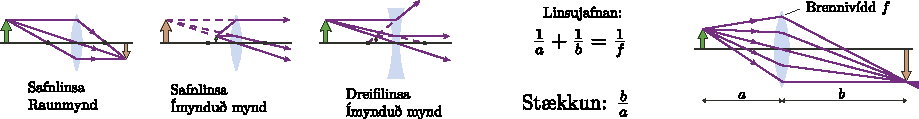
\includegraphics{figures/geislagangur.pdf}
\end{figure}
\begin{comment}
Helstu reglur til þess að teikna geislagangsmyndir:
\begin{enumerate}
    \item Geisli sem kemur samsíða inn í safnlinsu endar í brennipunkti linsunnar hinum meginn.
    \item Geisli sem kemur samsíða inn í dreifilinsu yfirgefur hana eins og úr brennipunktinum.
    \item Geisli sem fer í gegnum miðjuna á safnlinsu/dreifilinsu fer beint í gegn án stefnubreytingar.
    \item Geisli sem að kemur úr brennipunkti safnlinsu yfirgefur hana samsíða ás hennar.
    \item Geisli sem að stefnir á brennipunkt dreifilinsu yfirgefur hana samsíða ás hennar.
\end{enumerate}
\end{comment}
\end{tcolorbox}

\begin{enumerate}[label = \textbf{(\alph*)}]


\item[\textbf{(34.33)}] Hlutur sem er \SI{2.0}{cm} hár er staddur í \SI{30}{cm} fjarlægð frá safnlinsu sem hefur \SI{20}{cm} brennivídd. Teiknið geislagangsmynd og ákvarðið bæði fjarlægð eftirmyndarinnar frá safnlinsunni og hæð hennar.

\item[\textbf{(34.35)}] Hlutur sem er \SI{2.0}{cm} hár er staddur í \SI{12}{cm} fjarlægð frá safnlinsu sem hefur \SI{20}{cm} brennivídd. Teiknið geislagangsmynd og ákvarðið bæði fjarlægð eftirmyndarinnar frá safnlinsunni og hæð hennar.

\item[\textbf{(34.69)}] Ljósapera er stödd í \SI{3.0}{m} fjarlægð frá vegg. Í hvaða fjarlægð, $a$, frá ljósaperunni ættum við að setja safnlinsu með brennivídd, $f$, til þess að myndin sem að kemur fram á veggnum er tvisvar sinnum stærri heldur en fyrirmynd perunnar? (Ákvarðið bæði $a$ og $f$ þannig að þetta gangi).

\item[\textbf{(34.73)}] Þegar safnlinsu er komið fyrir \SI{10}{cm} fyrir framan hlut þá kemur fram upprétt, ímynduð mynd, sem er tvisvar sinnum stærri heldur en hluturinn sjálfur. Síðan færum við linsuna meðfram sama ás þar til að við sjáum viðsnúna raunmynd sem er tvisvar sinnum stærri heldur en hluturinn sjálfur. Um hversu langa vegalengd þurftum við að færa safnlinsuna?

\end{enumerate}

\begin{tcolorbox}
\begin{enumerate*}[label = ]
  \item \textbf{(34.33)} $\SI{60}{cm}$, $\SI{4.0}{cm}$.
  \item \textbf{(34.35)} $\SI{30}{cm}$, $\SI{5.0}{cm}$.
  \item \textbf{(34.69)} $a = \SI{1.0}{m}$, $f = \SI{67}{cm}$.
  \item \textbf{(34.73)} $\SI{20}{cm}$.
\end{enumerate*}
\end{tcolorbox}

\vspace{2cm}

\textbf{Bónusdæmi (Krotov 4.2.)} Augnlæknir nokkur ætlar að skoða augun í Matta nærsýna aðeins betur. Læknirinn stillir upp safnlinsu með \SI{9.0}{cm} brennivídd í \SI{36}{cm} fjarlægð frá auganu hans Matta og biður hann að um að horfa í gegn um linsuna (augnlæknirinn ætlar síðan að horfa hinum meginn frá á augun í Matta). Í hvaða fjarlægð ætti augnlæknirinn að vera til þess að sjá skarpa mynd af auganu hans Matta? Ef augun hans Matta hafa $\SI{24}{mm}$ þvermál, hversu stór sýnist augnlækninunum augun hans vera þegar að hann horfir í gegnum linsuna? Er þetta heppileg uppstilling? Hvað sér Matti augun á lækninum vera stór?

\vspace{0.3cm}

\textbf{Svar:} Læknirinn sér augun hans Matta vera \SI{8}{mm} að þvermáli í \SI{12}{cm} fjarlægð fyrir aftan safnlinsuna en Matti sér þvermálið á augum læknisins vera \SI{72}{mm}. Þeir ættu kannski að skipta um sæti!

\newpage

